% Generated from the public primitive catalog. Original Atlas drawing; Apache-2.0.
% Target: sm4-128; view: overview
\documentclass[border=9pt]{standalone}
% Original Atlas figure theme. Apache-2.0; see the repository LICENSE.
\usepackage[T1]{fontenc}
\usepackage{lmodern}
\usepackage{amsmath,amssymb}
\usepackage{tikz}
\usetikzlibrary{arrows.meta,positioning,calc,fit,backgrounds,decorations.pathreplacing,matrix}
\definecolor{atlasInk}{HTML}{172235}
\definecolor{atlasTeal}{HTML}{0D7B7D}
\definecolor{atlasMuted}{HTML}{637278}
\definecolor{atlasFill}{HTML}{EAF4F2}
\definecolor{atlasLine}{HTML}{B6C8C7}
\tikzset{
  every picture/.style={line width=.65pt,draw=atlasInk,>=Latex},
  every node/.style={text=atlasInk,font=\sffamily\small},
  box/.style={draw,rounded corners=1.5pt,minimum height=.9cm,minimum width=1.6cm,align=center,inner sep=6pt,fill=white},
  accent/.style={box,draw=atlasTeal,fill=atlasFill},
  wire/.style={->,line width=.7pt},
  keywire/.style={wire,draw=atlasTeal,dashed},
  xor/.style={draw,circle,fill=white,inner sep=0pt,minimum size=.38cm},
  add/.style={draw,rectangle,fill=white,inner sep=0pt,minimum size=.38cm},
  note/.style={font=\sffamily\scriptsize,text=atlasMuted,align=center},
  phase/.style={font=\sffamily\small\bfseries,text=atlasTeal},
  group/.style={draw=atlasLine,dashed,rounded corners=2pt,inner sep=8pt}
}
\newcommand{\rotl}{\mathbin{\lll}}
\newcommand{\rotr}{\mathbin{\ggg}}
\newcommand{\kx}{\operatorname{Keccak}\!\text{-}\!f[1600]}

\newcommand{\AtlasKeyBits}{128}
\newcommand{\AtlasKeyWords}{4}
\newcommand{\AtlasRounds}{32}
\newcommand{\AtlasPriorRounds}{31}
\newcommand{\AtlasRoundKeys}{33}
\newcommand{\AtlasDoubleRounds}{16}
\newcommand{\AtlasSixRoundGroups}{5.333333333333333}
\newcommand{\AtlasFLGroups}{4.333333333333333}
\newcommand{\AtlasRoundStart}{-8}
\newcommand{\AtlasBlockBits}{128}
\newcommand{\AtlasOutputBits}{d}
\newcommand{\AtlasStateBits}{8w}
\newcommand{\AtlasNonceBits}{v}
\newcommand{\AtlasCounterBits}{q}
\newcommand{\AtlasStreamBlockBits}{b}
\newcommand{\AtlasRate}{r}
\newcommand{\AtlasCapacity}{c}
\newcommand{\AtlasSteps}{N}
\newcommand{\AtlasLastStep}{N-1}
\newcommand{\AtlasWordBits}{w}
\newcommand{\AtlasHashWords}{h}
\newcommand{\AtlasFeedForward}{\boxplus}
\newcommand{\AtlasByteOrder}{big-endian}
\newcommand{\AtlasDomain}{01}
\newif\ifAtlasXof
\AtlasXoffalse
\begin{document}
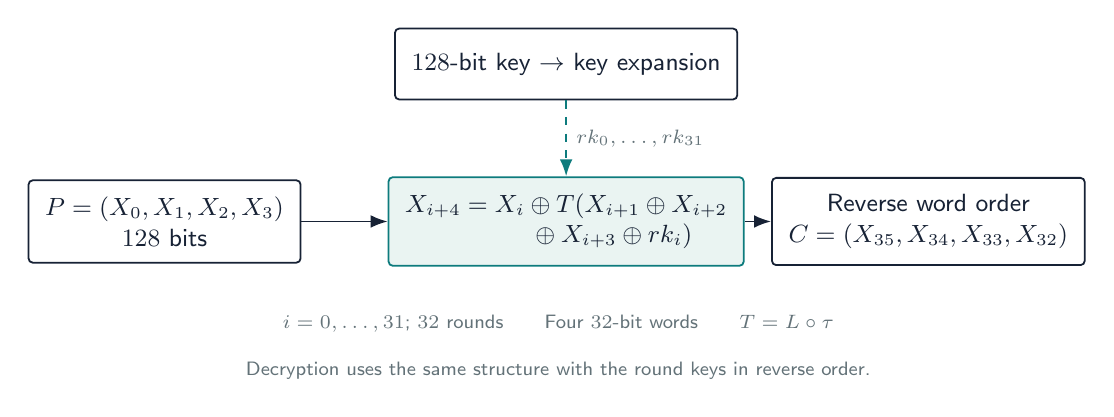
\begin{tikzpicture}
  \node[box] (in) at (0,0) {$P=(X_0,X_1,X_2,X_3)$\\$\AtlasBlockBits$ bits};
  \node[accent,minimum width=4.5cm] (rounds) at (5.1,0) {$X_{i+4}=X_i\oplus T(X_{i+1}\oplus X_{i+2}$\\$\phantom{X_{i+4}={}}\oplus X_{i+3}\oplus rk_i)$};
  \node[box] (reverse) at (9.7,0) {Reverse word order\\$C=(X_{35},X_{34},X_{33},X_{32})$};
  \draw[wire] (in) -- (rounds); \draw[wire] (rounds) -- (reverse);
  \node[box] (schedule) at (5.1,2) {$\AtlasKeyBits$-bit key $\to$ key expansion};
  \draw[keywire] (schedule) -- node[right,note] {$rk_0,\ldots,rk_{\AtlasPriorRounds}$} (rounds);
  \node[note] at (5,-1.3) {$i=0,\ldots,\AtlasPriorRounds$; $\AtlasRounds$ rounds\qquad Four $32$-bit words\qquad $T=L\circ\tau$};
  \node[note] at (5,-1.9) {Decryption uses the same structure with the round keys in reverse order.};
\end{tikzpicture}

\end{document}
